Para o experimento de medição do tempo de conexão de equipamentos de usuário, foi levado em consideração o tempo total entre o início do processo de registro e a obtenção do plano de dados. Após a coleta e processamento dos dados desse experimento, os gráficos da Figura \ref{fig:exp1_conn} foram gerados para permitir a visualização e análise dos dados coletados.
O gráfico representa o tempo médio de conexão para cada rajada de conexões simultâneas, com o eixo X representando o tempo de execução do experimento, em segundos, e o eixo Y representando o tempo total para estabelecer a conexão e iniciar o plano de dados deste equipamento de usuário, em milissegundos.
Na coluna da esquerda, são apresentados os resultados para o núcleo 5G \textit{free5GC} e, na direita, o \textit{Open5GS}. Para cada núcleo, foram desenhados 5 gráficos, com as diferentes variações de intervalo entre rajadas de conexões de UEs.

Ao analisar os dados, é possível inferir que, para as condições do experimento, o núcleo \textit{free5GC} possuiu tempo de conexão médio de 1089 ms, quando cada conexão se iniciou 500 ms após a anterior.
Nesse experimento, a mediana do tempo de conexão foi de 853 ms e o tempo máximo de conexão foi de 5,57 segundos.
Para um intervalo entre conexões de 100 ms, o tempo médio de conexão foi de 7731 ms, tendo sua mediana em 3027 ms e o tempo máximo de conexão durando pouco mais de 54 segundos.

Quanto ao comportamento do núcleo de rede 5G \textit{Open5GS}, percebe-se que para um intervalo de 500 ms, o tempo médio foi de 306 ms, com sua mediana em 305 ms e seu tempo máximo de conexão em 345 ms.
Para o intervalo de 100 ms, a média subiu para 364 ms, enquanto a mediana subiu para 358 ms e o valor máximo atingiu 490 ms.
Desse modo, considerando-se apenas o tempo de conexão, o núcleo de rede \textit{Open5GS} possui melhor desempenho, aguentando diversas rajadas de conexões em diferentes cenários, tendo seu tempo médio variando em torno de 58 milissegundos. O núcleo \textit{free5GC} possui uma variação de aproximadamente 49 segundos entre as diferentes execuções do experimento.
Os dados detalhados para cada execução desse experimento podem ser vistos na Tabela \textcolor{red}{INSERIR TABELA}.

\begin{figure}[H]
    \centering
    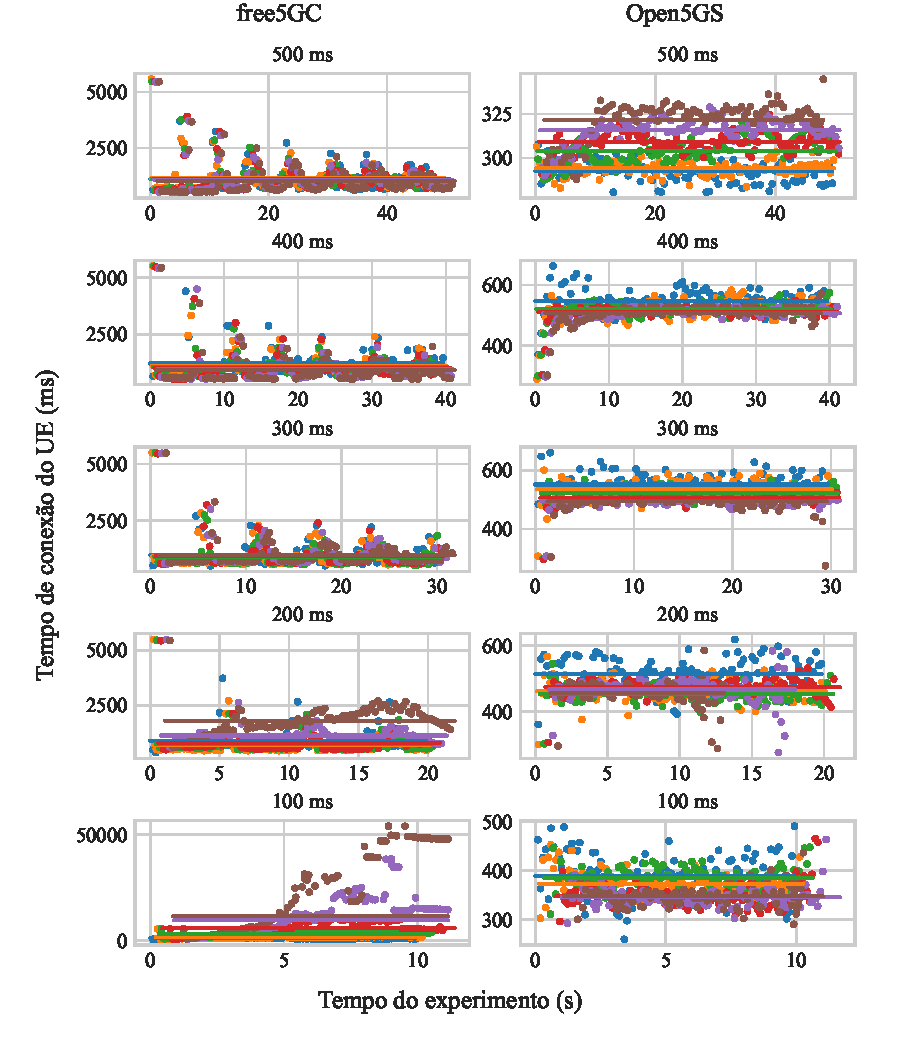
\includegraphics[width=0.85\textwidth]{TG2/Chapters/DataAnalysis/Figures/EXP1-CONN-12C-8GB.pdf}
    \caption{Tempo de registro e estabelecimento de sessão PDU para cada núcleu 5G}
    \label{fig:exp1_conn}
\end{figure}

Durante a execução dos experimentos, a taxa de conexões mal sucedidas entre o UE e o núcleo da rede foi significativa entre cada execução do experimento para cada um dos núcleos testados. Sendo assim, foi desenhado os gráficos da Figura \ref{fig:exp1_conn_err} com a comparação de taxa de erro média entre os dois núcleos avaliados.
Cada gráfico representa a taxa de erro média de conexão dos UEs com os núcleos testados, com o intervalo de tempo entre as rajadas em ordem decrescente, de 500 a 100 ms, com passos de 100 ms.
As barras dos gráficos representam a média de erros entre as execuções do experimento realizadas para cada configuração de gNB e núcleo, enquanto as linhas representam o desvio padrão da média para cada execução do experimento.

Nesse experimento, foi possivel observar que o núcleo \textit{free5GC} possui uma taxa de erros de conexão crescente para cada gNB adicionada. Ao adicionar uma gNB, a taxa de conexões simultâneas aumentava na mesma proporção que a taxa de erros.
Esse comportamento pode ser percebido no núcleo \textit{Open5GS} quando se reduz o intervalo entre rajadas de conexões para um valor menor que o tempo médio necessário para se estabelecer a conexão.
Entretanto, para intervalos maiores de tempo, o núcleo \textit{Open5GS} apresentou boa estabilidade no geral, tendo em alguns momentos a taxa de erros de conexão igual a zero.

Através da análise desses resultados, percebe-se que o núcleo de rede 5G \textit{Open5GS} possui maior estabilidade para o registro de sessões dos UE em escala em comparação com o núcleo \textit{free5GC}.
Apesar desses resultados, foi descoberta uma limitação no núcleo \textit{Open5GS} em relação à quantidade máxima de dispositivos conectados simultaneamente, sendo essa igual a 1024 dispositivos.
É importante ressaltar que essa limitação não está presente no núcleo \textit{free5GC}.
Os dados detalhados para cada execução desse experimento podem ser vistos na Tabela \textcolor{red}{INSERIR TABELA - TALVEZ SEJA A MESMA DE CIMA}.

\begin{figure}[H]
    \centering
    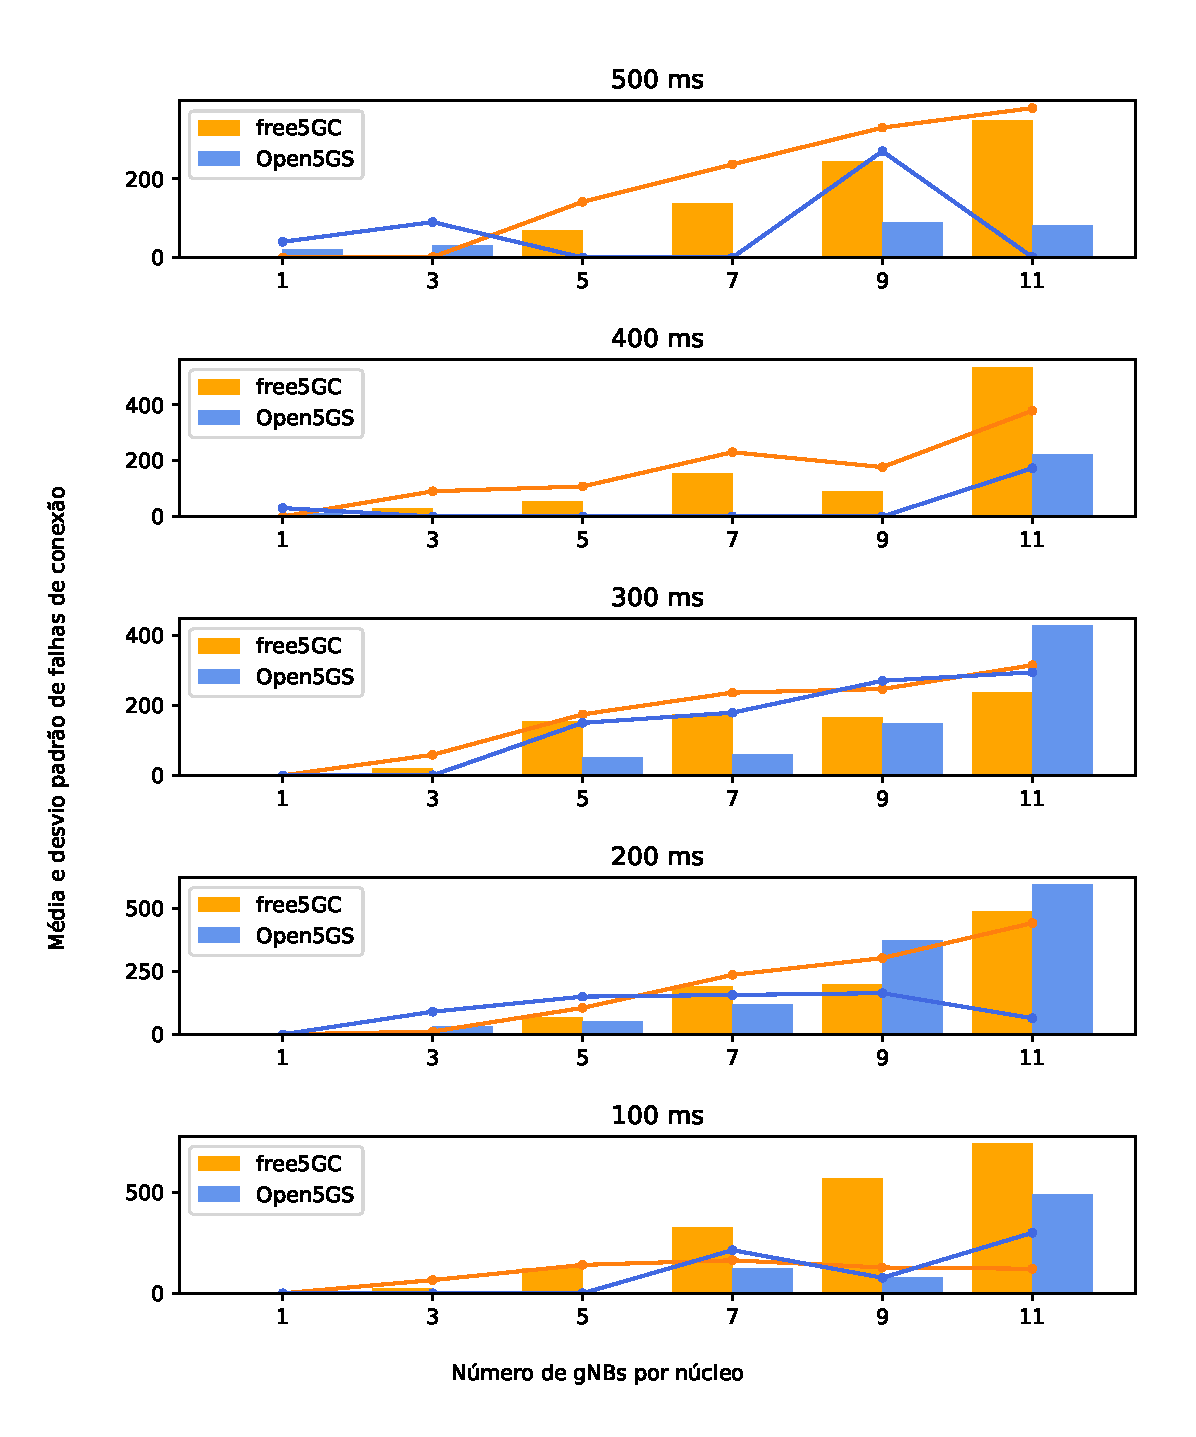
\includegraphics[width=0.95\textwidth]{TG2/Chapters/DataAnalysis/Figures/EXP1-CONN_ERR-12C-8GB.pdf}
    \caption{Média e desvio padrão dos erros de conectividade nos experimentos executados}
    \label{fig:exp1_conn_err}
\end{figure}
